\section{Design of the Solution}
\label{sec:design-of-the-solution}


The high-level concepts of our solution consist in splitting the infrastructure in \textbf{hierarchical levels} and allowing the developers to specify on which levels the clients save and access the data.
\\Our API allows to:
\begin{itemize}
    \item Specify the \textbf{hierarchy} of the infrastructure, in serverless setups this should be done by the web infrastructure companies;
    \item Deploy \textbf{geo-distributed functions} exactly where needed;
    \item Have a \textbf{geographically-partitioned stateful support}, where each location (e.g., the cloudlet in a city) has its own set of data;
    \item \textbf{Save data easily} by only specifying one or multiple levels, then the actual location is obtained by the framework.
\end{itemize}

These concepts allow a lot of versatility where the developer can process the data at a certain level and then organize the results in geographic partitions, without actually specifying where to save the results, but only specifying the levels and letting the framework handle the rest.

\begin{figure}
    \centering
    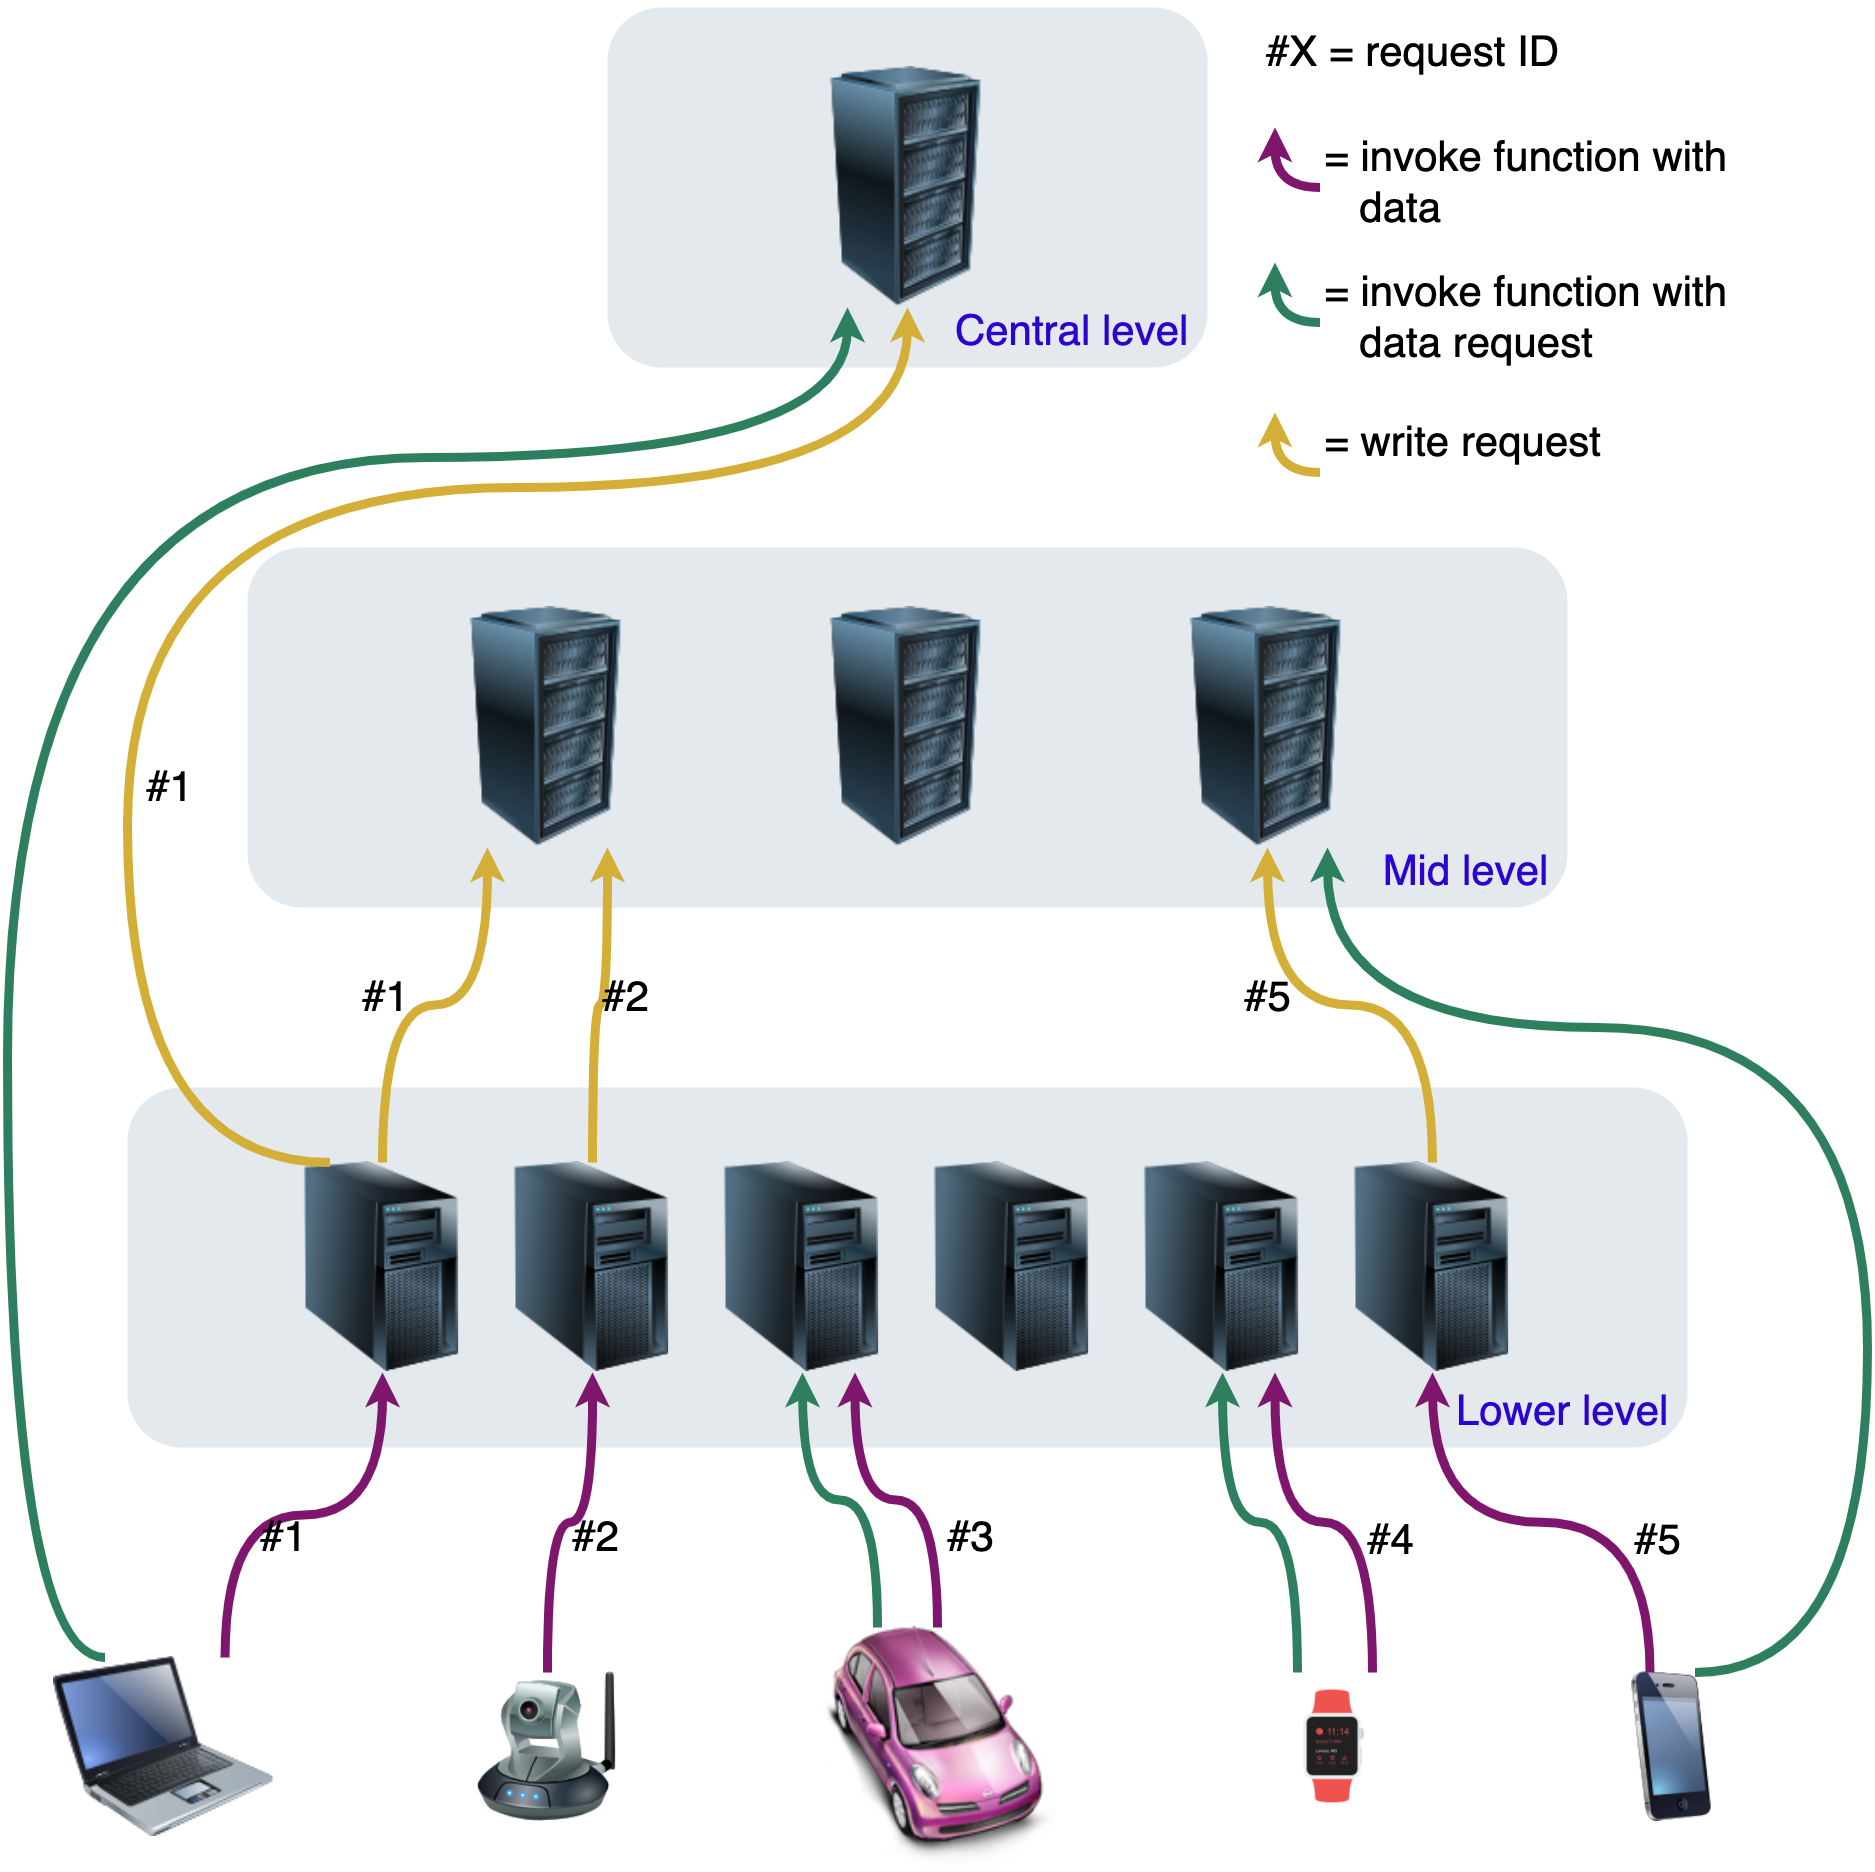
\includegraphics[width=0.99\linewidth]{Figures/Solution/high-level-architecture.png}
    \caption{High-level architecture of an example setup}
    \label{fig:high-level-architecture}
\end{figure}

In Figure \ref{fig:high-level-architecture} we show an example with three levels. Clients can \textbf{invoke functions} on the nearest location of a certain level, these functions can be used for both \textbf{sending data} or \textbf{requesting data}. When clients send data, the function written by the developer can process the data and then save the results in the provided stateful support. The results can be saved on different and multiple levels.


\subsection{Finding the Nearest Location}
Our solution assumes the presence of the ability to contact the \textbf{nearest server} automatically, without the intervention of the developer (the developer just needs to send the request to the function's URL).

This process has already been proved to be feasible and is in fact exploited by many web infrastructure companies to provide a Content Delivery Network or to provide serverless edge computing. The most common procedures to perform the process are the following:
\begin{itemize}
    \item \textbf{Anycast Routing}: this routing procedure uses the Border Gateway Protocol (BGP) to route clients using the natural network flow, indeed the information collected by the BGP protocol about network neighbors is used to efficiently route traffic based on hop count ensuring the shortest traveling distance between the client and its final destination \cite{anycast-cloudflare}.
    \item \textbf{Unicast Routing}: a process which can be incorporated into the standard Domain Name System (DNS) resolution process by using recursive DNS queries which redirect clients to the server closest to the DNS resolver (and usually the DNS resolver is physically near the client) \cite{unicast-vs-anycast}.
    \item \textbf{Manual Routing}: a procedure in which the client computes on its own which is the most appropriate server to contact, with this procedure GPS-equipped devices can use more precise information about the location.
\end{itemize}

In the implementation of our prototype we use a Manual Routing procedure where the clients would manually contact the nearest server, but in a real scenario a process like Unicast Routing or Anycast Routing could be preferred.


\subsection{Suitable Use Cases}
Our solution, for how has been thought, is suitable for use cases with the following characteristics:
\begin{itemize}
    \item \textbf{Stateful computation}: the use case needs a stateful support with \textbf{frequent writes} and reads.
    \item \textbf{Location awareness}: the use cases works on \textbf{geographic partitions} of the data;
    \item \textbf{Location is static}: data producers do not change location; OR \textbf{Location is dynamic but it’s not a problem to have a discontinuity in the data}: e.g., if there is an aggregation at the "city" level and a data producer exits the city, its data will have a discontinuity;
    \item \textbf{Session consistency is not needed}: the concept of session, where the user maintains consistency of the data even when the connected server changes, is not provided by our solution;
\end{itemize}
